% !TEX TS-program = pdflatex
% !TEX encoding = UTF-8 Unicode

% This is a simple template for a LaTeX document using the "article" class.
% See "book", "report", "letter" for other types of document.

\documentclass[11pt]{article} % use larger type; default would be 10pt

\usepackage[utf8]{inputenc} % set input encoding (not needed with XeLaTeX)

%%% Examples of Article customizations
% These packages are optional, depending whether you want the features they provide.
% See the LaTeX Companion or other references for full information.

%%% PAGE DIMENSIONS
\usepackage{geometry} % to change the page dimensions
\geometry{a4paper} % or letterpaper (US) or a5paper or....
% \geometry{margin=2in} % for example, change the margins to 2 inches all round
% \geometry{landscape} % set up the page for landscape
%   read geometry.pdf for detailed page layout information

\usepackage{graphicx} % support the \includegraphics command and options
\graphicspath{ {./Figs/} }  % requires additional {} and trailing '/'!


% \usepackage[parfill]{parskip} % Activate to begin paragraphs with an empty line rather than an indent

%%% PACKAGES
\usepackage{booktabs} % for much better looking tables
\usepackage{array} % for better arrays (eg matrices) in maths
\usepackage{paralist} % very flexible & customisable lists (eg. enumerate/itemize, etc.)
\usepackage{verbatim} % adds environment for commenting out blocks of text & for better verbatim
\usepackage{subfig} % make it possible to include more than one captioned figure/table in a single float

\usepackage{colortbl}

\usepackage{amsmath}
\usepackage{xifthen}
\usepackage{tikz}
\usepackage{relsize}
\usetikzlibrary{matrix}
\usetikzlibrary{positioning}
\usetikzlibrary{calc}
\usetikzlibrary{shapes}

\usepackage{theorem}
\newtheorem{definition}{Definition}


% These packages are all incorporated in the memoir class to one degree or another...

%%% HEADERS & FOOTERS
\usepackage{fancyhdr} % This should be set AFTER setting up the page geometry
\pagestyle{fancy} % options: empty , plain , fancy
\renewcommand{\headrulewidth}{0pt} % customise the layout...
\lhead{}\chead{}\rhead{}
\lfoot{}\cfoot{\thepage}\rfoot{}

%%% SECTION TITLE APPEARANCE
\usepackage{sectsty}
\allsectionsfont{\sffamily\mdseries\upshape} % (See the fntguide.pdf for font help)
% (This matches ConTeXt defaults)

%%% ToC (table of contents) APPEARANCE
\usepackage[nottoc,notlof,notlot]{tocbibind} % Put the bibliography in the ToC
\usepackage[titles,subfigure]{tocloft} % Alter the style of the Table of Contents
\renewcommand{\cftsecfont}{\rmfamily\mdseries\upshape}
\renewcommand{\cftsecpagefont}{\rmfamily\mdseries\upshape} % No bold!

%%% END Article customizations

\newcommand{\ub}{\text{{\tt.}}}

\tikzstyle{bp}=[line width=5pt,draw=blue, opacity=.6,in =90,out=90,looseness=1.5]
\tikzstyle{altbp}=[line width=5pt,draw=red, opacity=.6, in =-90,out=-90,looseness=1.5]
\tikzstyle{cell}=[inner sep=2]
\tikzstyle{backbone}=[line width=2pt]
\tikzstyle{every picture}+=[remember picture]

\def\mySecStr#1{\expandafter {\tt #1}\& }
\def\mySecStrAll#1{\ifx#1\mySecStrAll\else\mySecStr#1\expandafter\mySecStrAll\fi}
\def\mySeq#1{\expandafter {\relsize{-2}\sf #1}\&}
\def\mySeqAll#1{\ifx#1\mySeqAll\else\mySeq#1\expandafter\mySeqAll\fi}


\newcommand{\RNA}[3][]{
\begin{tikzpicture}[baseline={([yshift=-.5ex]rna)}]
  \matrix[matrix of nodes,nodes=cell,ampersand replacement=\&] (rna){
		\mySecStrAll #2 \mySecStrAll\\
		};
\ifthenelse{\equal{#3}{}}{}{%
	\foreach \x/\y in {#3}{\draw (rna-1-\x) edge[bp] (rna-1-\y);}%
}
\ifthenelse{\equal{#1}{}}{}{%
		\foreach \x/\y in {#1}{\draw (rna-1-\x) edge[altbp] (rna-1-\y);}%
		}
\end{tikzpicture}} 

\setlength{\parskip}{1em}
\renewcommand{\H}[1]{{\tt#1}}


\newcommand{\Summary}{
  \tikzstyle{bp}=[line width=5pt,draw=red!50!blue, opacity=.6,in =90,out=90,looseness=1.5]
  \tikzstyle{altbp}=[line width=5pt,draw=red!50!blue, opacity=.6, in =90,out=90,looseness=1.5]
}


\newcommand{\Case}[3]{\item $\{#1\}$: {\sf #3}-type

{\centering 
#2 $\longrightarrow$\Summary#2\\}

}


%%% The "real" document content comes below...

\title{A first step towards an unambiguous DP scheme for CCJ}
\author{Hosna, Sebastian, Yann}
%\date{} % Activate to display a given date or no date (if empty),
         % otherwise the current date is printed 

\begin{document}
\maketitle


The original DP decomposition underlying the CCJ algorithm is ambiguous on multiple levels.
{\em Can we lift this ambiguity without too much hassle?}
A key element in the decomposition, and one of the major source of ambiguity, resides in the assembly of two \emph{gapped} pseudoknotted elements, akin to the 3-band/kissing hairpin motif. However, in order to achieve maximum expressivity, only the middle helix is mandatory within each gapped element, meaning that some structure may be obtained in several different ways. In this short note, we explore the different combinations, and build a minimal subset of structures, built from combinations of atomic gapped structures that captures the same search space within inducing any ambiguity.

Let us first introduce a bit of nomenclature. The helices in the first gapped structure are named \H{1}, \H{2} and \H{3} (resp. \H{A}, \H{B} and \H{C}), as illustrated below:

{\centering 
\RNA[4/6,5/11,10/12]{121ABA323CBC}{1/3,2/8,7/9}\\}

\noindent Note that each helix must contain at least one base pair and, in the case where it contains internal loops and recursive subtructures\footnote{Are those allowed anyway?} must start and finish with a base pair (potentially the same if restricted to a single base pair).

In order to avoid ambiguity at a higher level in the decomposition, it is crucial that the base pairs in the assembly of gapped elements form a unique connected component in the conflict graph induced by the crossing relationship. Indeed, disconnected components correspond to part in a pseudoknot that can be generated either by sequential composition, or by a recursive call, generating a nested subcomponent. It is thus easy to say that helices \H{2} and \H{B} cannot be omitted. Conversely, helices \H{1}, \H{3}, \H{A}, and \H{C} represent leaves of the conflict graph, and can therefore be safely discarded without disconnecting the conflict graph, \emph{i.e.} without inducing any ambiguity.

We are left to systematically explore the subsets of $\{\H{1}, \H{3}, \H{A}, \H{C}\}$, in combination with the two mandatory helices \H{2} and \H{B}:
\begin{itemize} 
\item Second component is $\{\H{B}\}$:
\begin{itemize} 
\Case{\H{2}, \H{B}}{\RNA[5/11]{-2--B--2--B-}{2/8}}{H}
\Case{\H{1},\H{2}, \H{B}}{\RNA[5/11]{121-B--2--B-}{1/3,2/8}}{KH}
\Case{\H{2}, \H{3}, \H{B}}{\RNA[5/11]{-2--B-323-B-}{2/8,7/9}}{H}
{\bfseries Note:} Second band features at least 2 base pairs
\Case{\H{1},\H{2}, \H{3}, \H{B}}{\RNA[5/11]{121-B-323-B-}{1/3,2/8,7/9}}{KH}
{\bfseries Note:} Third band features at least 2 base pairs
\end{itemize} 
\item Second component is $\{\H{A},\H{B}\}$:
\begin{itemize} 
\Case{\H{2}, \H{A}, \H{B}}{\RNA[4/6,5/11]{-2-ABA-2--B-}{2/8}}{H}
{\bfseries Note:} First band features at least 2 base pairs
\Case{\H{1},\H{2}, \H{A}, \H{B}}{\RNA[4/6,5/11]{121ABA-2--B-}{1/3,2/8}}{KH$^{\text{a}}$}
\Case{\H{2}, \H{3}, \H{A}, \H{B}}{\RNA[4/6,5/11]{-2-ABA323-B-}{2/8,7/9}}{H$^{\text{a}}$}
\Case{\H{1},\H{2}, \H{3}, \H{A}, \H{B}}{\RNA[4/6,5/11]{121ABA323-B-}{1/3,2/8,7/9}}{KH$^{\text{b}}$}
\end{itemize} 
\item Second component is $\{\H{B},\H{C}\}$:
\begin{itemize} 
\Case{\H{2}, \H{B}, \H{C}}{\RNA[5/11,10/12]{-2--B--2-CBC}{2/8}}{KH}
\Case{\H{1},\H{2}, \H{B}, \H{C}}{\RNA[5/11,10/12]{121-B--2-CBC}{1/3,2/8}}{4B}
\Case{\H{2}, \H{3}, \H{B}, \H{C}}{\RNA[5/11,10/12]{-2--B-323CBC}{2/8,7/9}}{KH$^{\text{c}}$}
\Case{\H{1},\H{2}, \H{3}, \H{B}, \H{C}}{\RNA[5/11,10/12]{121-B-323CBC}{1/3,2/8,7/9}}{4B$^{\text{a}}$}
\end{itemize} 
\item Second component is $\{\H{A},\H{B},\H{C}\}$:
\begin{itemize} 
\Case{\H{2}, \H{A}, \H{B}, \H{C}}{\RNA[4/6,5/11,10/12]{-2-ABA-2-CBC}{2/8}}{KH}
{\bfseries Note:} First band features at least 2 base pairs
\Case{\H{1},\H{2}, \H{A}, \H{B}, \H{C}}{\RNA[4/6,5/11,10/12]{121ABA-2-CBC}{1/3,2/8}}{4B$^{\text{b}}$}
\Case{\H{2}, \H{3}, \H{A}, \H{B}, \H{C}}{\RNA[4/6,5/11,10/12]{-2-ABA323CBC}{2/8,7/9}}{KH$^{\text{d}}$}
\Case{\H{1},\H{2}, \H{3}, \H{A}, \H{B}, \H{C}}{\RNA[4/6,5/11,10/12]{121ABA323CBC}{1/3,2/8,7/9}}{CCJ}
\end{itemize}
\end{itemize}

\begin{table}
{ 
  \tikzstyle{cell}=[inner sep=1.2]
  \tikzstyle{bp}=[line width=2pt,draw=red!50!blue!80!white, opacity=1,in =90,out=90,looseness=1.3]
  \tikzstyle{altbp}=[line width=2pt,draw=red!50!blue!80!white, opacity=1, in =90,out=90,looseness=1.3]
\centering\begin{tabular}{@{}ll@{}ll@{}l@{}}\toprule
Type & Helix classes && Subsets (sort of)&\\ \midrule
{\sf H} & $\{\H{2},\H{B}\}$ &\RNA[5/11]{-2--B--2--B-}{2/8}& $\{\H{2},\H{3},\H{B}\}$&\RNA[5/11]{-2--B-323-B-}{2/8,7/9}\\ 
& &  & $\{\H{2},\H{A},\H{B}\}$  &\RNA[4/6,5/11]{-2-ABA-2--B-}{2/8}\\ 
\arrayrulecolor{gray!60}\midrule
{\sf H}$^{\text{a}}$ & $\{\H{2}, \H{3}, \H{A}, \H{B}\}$&\RNA[4/6,5/11]{-2-ABA323-B-}{2/8,7/9} &  &\\ 
\arrayrulecolor{black}\midrule
{\sf KH} & $\{\H{1},\H{2},\H{B}\}$&\RNA[5/11]{121-B--2--B-}{1/3,2/8} & $\{\H{1},\H{2},\H{3},\H{B}\}$  &\RNA[5/11]{121-B-323-B-}{1/3,2/8,7/9}\\ 
 & $\{\H{2},\H{B},\H{C}\}$ &\RNA[5/11,10/12]{-2--B--2-CBC}{2/8} & $\{\H{2},\H{A},\H{B},\H{C}\}$  &\RNA[4/6,5/11,10/12]{-2-ABA-2-CBC}{2/8}\\ 
\arrayrulecolor{gray!60}\midrule
{\sf KH}$^{\text{a}}$ & $\{\H{1},\H{2}, \H{A}, \H{B}\}$&\RNA[4/6,5/11]{121ABA-2--B-}{1/3,2/8} &  & \\ 
{\sf KH}$^{\text{b}}$ & $\{\H{1},\H{2}, \H{3}, \H{A}, \H{B}\}$&\RNA[4/6,5/11]{121ABA323-B-}{1/3,2/8,7/9} &  &\\ 
{\sf KH}$^{\text{c}}$ & $\{\H{2}, \H{3}, \H{B}, \H{C}\}$&\RNA[5/11,10/12]{-2--B-323CBC}{2/8,7/9} &  & \\ 
{\sf KH}$^{\text{d}}$ & $\{\H{2}, \H{3}, \H{A}, \H{B}, \H{C}\}$&\RNA[4/6,5/11,10/12]{-2-ABA323CBC}{2/8,7/9} &  & \\ 
\arrayrulecolor{black}\midrule
{\sf 4B} & $\{\H{1},\H{2},\H{B},\H{C}\}$&\RNA[5/11,10/12]{121-B--2-CBC}{1/3,2/8}  &  &\\ 
\arrayrulecolor{gray!60}\midrule
{\sf 4B}$^{\text{a}}$ & $\{\H{1},\H{2}, \H{3}, \H{B}, \H{C}\}$&\RNA[5/11,10/12]{121-B-323CBC}{1/3,2/8,7/9} &  & \\ 
{\sf 4B}$^{\text{b}}$ & $\{\H{1},\H{2}, \H{A}, \H{B}, \H{C}\}$&\RNA[4/6,5/11,10/12]{121ABA-2-CBC}{1/3,2/8} &  & \\ 
\arrayrulecolor{black}\midrule
{\sf CCJ} & $\{\H{1},\H{2},\H{3},\H{A},\H{B},\H{C}\}$&\RNA[4/6,5/11,10/12]{121ABA323CBC}{1/3,2/8,7/9} &  &\\ 
\bottomrule
\end{tabular}\\}

\caption{Isomorphism classes for relevant subsets of {\sf CCJ} helices}\label{tab:iso}
\end{table}

We summarize in Table~\ref{tab:iso} the various accessible classes. A close inspection of the classes reveals two -- complete and unambiguous -- decompositions of the CCJ class in the following subsets of non-empty helices:

{\centering$\{\H{2},\H{B}\}$, 
$\{\H{2}, \H{3}, \H{A}, \H{B}\}$, 
$\{\H{1},\H{2},\H{B}\}$ \emph{or} $\{\H{2},\H{B},\H{C}\}$,
$\{\H{1},\H{2}, \H{A}, \H{B}\}$,
$\{\H{1},\H{2}, \H{3}, \H{A}, \H{B}\}$,
$\{\H{2}, \H{3}, \H{B}, \H{C}\}$,
$\{\H{2}, \H{3}, \H{A}, \H{B}, \H{C}\}$,
$\{\H{1},\H{2},\H{B},\H{C}\}$,
$\{\H{1},\H{2}, \H{3}, \H{B}, \H{C}\}$,
$\{\H{1},\H{2}, \H{A}, \H{B}, \H{C}\}$,
$\{\H{1},\H{2},\H{3},\H{A},\H{B},\H{C}\}$\\}

From this partition of the search space for canonical CCJ pseudoknots, one obtains a complete/unambiguous, if definitely tedious, decomposition:
\newcommand{\Basic}{
  \tikzstyle{bp}=[line width=20pt,draw=blue!50!red!80, opacity=.6, in=90, out=90,looseness=2]
  \tikzstyle{altbp}=[line width=20pt,draw=blue!50!red!80, opacity=.6, in=-90, out=-90,looseness=2]
  \tikzstyle{cell}+=[inner sep=8pt]
}
\newcommand{\RHS}[2]{{\Basic
  \tikzstyle{bp}+=[draw=blue]
  \tikzstyle{altbp}+=[draw=red]
\RNA[2/4]{----}{1/3}
\tikz[overlay]{
\node[above=17.5pt of rna-1-2,inner sep=2pt,fill=blue!10,rounded corners=3pt]{\H{#1}};
\node[below=17.5pt of rna-1-3,inner sep=2pt,fill=red!10,rounded corners=3pt]{\H{#2}};
\draw[backbone] (rna-1-1.west) edge (rna-1-4.east); 
\node[below=1pt of rna-1-1.north west,inner sep=0]{$i$};
\node[below=1pt of rna-1-1.north east,inner sep=0]{$k$};
\node[above=1pt of rna-1-2.south west,inner sep=0]{$k$+$1$};
\node[above=1pt of rna-1-2.south east,inner sep=0]{$l$};
\node[below=1pt of rna-1-3.north west,inner sep=0]{$l$+$1$};
\node[below=1pt of rna-1-3.north east,inner sep=0]{$m$};
\node[above=1pt of rna-1-4.south west,inner sep=0]{$m$+$1$};
\node[above=1pt of rna-1-4.south east,inner sep=0]{$j$};

}}}
\begin{align*}
{\Basic\RNA[2/4]{----}{1/3}
\tikz[overlay]{
\node[below=-2pt of rna-1-1.south west,inner sep=0]{$i$};
\node[above=-2pt of rna-1-4.north east,inner sep=0]{$j$};
\draw[backbone] (rna-1-1.west) edge (rna-1-4.east); 
}}  \to &\RHS{2}{B} + \RHS{2,3}{A,B} + \RHS{1,2}{B}\\
+&\RHS{1,2}{A,B}+\RHS{1,2,3}{A,B}+\RHS{2,3}{B,C}\\
+&\RHS{2,3}{A,B,C}+\RHS{1,2}{B,C}+\RHS{1,2,3}{B,C}\\
+&\RHS{1,2}{A,B,C}+\RHS{1,2,3}{A,B,C}\\
\end{align*}
This decomposition must then be completed with rules for the \emph{gapped} portions, essentially corresponding to constrained versions of rules in the initial {\sf CCJ} algorithm.

\section{Unambiguous decomposition}

\subsection{Preliminaries}

\begin{definition}[band]
A \emph{band} is a set of base pairs that 1) are nested to each other, 2) all cross the same set of (other) base pairs.
Here, two base pairs $(i,j)$ and $(i',j')$ are \emph{nested} iff $i<i'<j'<j$ or $i'<i<j<j'$.
\end{definition}


\subsection{Methods}

Arbitrary CCJ-structures are decomposed unambiguosly due to
\begin{equation}

\includegraphics{KnottyPF/recursionW}
\end{equation}
Similar changes disambiguate the WB and WP recursions. 
This moves the focus to the decomposition of $P$-fragments. $P$-fragments represent structures $R$ of subsequences $i..l$, where
$i$ and $l$ are paired and part of the same pseudoknot, i.e. in all those structures, there are base pairs $(i,i')$ and $(l',l)$, such that
\begin{enumerate}
\item either $(i,i')$ and $(l',l)$ are crossing each other
\item or $(i,i')$ and $(l',l)$ are both crossing a third base pair $(k,k')$, where $i<k<i'<l'<k'<l$.
\item $(i,i')$ crosses a base pair $(k_1,k_1')$ that crosses $(k_2,k'_2)$ that crosses $(l',l)$ $(i<k_1<k_2<k'_1<k'_2<l)$.
\end{enumerate}
We observe that all these cases are disjoint and form a complete decomposition of CCJ structures, since CCJ structures do not allow three base pairs that all pairwise cross each other and the longest possible chains of crossing base pairs are $4$-chains (third case).

In each case, we decompose the $P$-fragment over [i..l] into two gapped fragments over $[i..j]\cup[k..k']$ and $[j+1..k-1]\cup[k'+1..l]$. 

%Gapped fragment: $\RNA{i-j----k-l}{1/10,3/8}$
%
%P-fragment decomposed into two gapped fragments: $\RNA{i-----------l}{1/10,3/8,4/13,7/11}$

For case 1, we achieve crossing of $(i,i')$ and $(l',l)$ if and only if the
base pairs 'span' the gap in their respective fragment. We define, in a gapped
fragment over $[i..j]\cup[k..l]$ ($i\leq j<k\leq l$), a base pair (x,y)
\emph{spans the gap} iff $x\in[i..j]$ and $y\in[k..l]$.

Case 3 applies iff in both gapped fragments, the respective base pairs $(i,i')$ and $(l',l)$ do not span the gap.

In the remaining case 2, one of the base pairs spans the gap and the other does
not. We can arbitrarily break the implied symmetry by requiring $(i,i')$ to
span the gap in its gapped fragment.

\paragraph{Types of gapped fragments}

First of all, note that the decomposition of a P-fragment, can be unambiguous
only, if we strengthen the requirements in the gapped fragments compared to the
PK-fragments of the ambiguous CCJ algorithm.  For the structures represented by
PK-type gapped fragments on $[i..j]\cup[k..l]$ we require that $i$, $j$ and $l$
are paired to respective positions $i'$, $j'$, $l'$. Moreover, each of these
base pairs either crosses one of the others.  Note that there are special
cases, where $i=j$ or $k=l$ or both. In these cases, there are only one or two
such base pairs, but the same conditions apply. Moreover, there must be one
base pair that spans the gap. (In comparison, the original CCJ algorithm
required similar conditions only for $i$ and $l$.)

Our considerations give raise to defining four types of gapped
fragments, where
\begin{enumerate}
\item $(i,i')$ spans the gap,
\item $(i,i')$ does not span the gap,
\item $(l',l)$ spans the gap,
\item $(l',l)$ does not span the gap.
\end{enumerate}

Note that this suffices to (de)compose the different types of P-fragments in
the disjoint case distinction that we discussed before.

We observe that the different types of gapped fragments can be distinguished by limiting
the possible decomposition orders in terms of decomposition at the bands L,R,M, and O.
E.g. the constraint (1) is ensured by not decomposing at the left band after the last decomposition at the O-band.
When we represent the band-decomposition order as word over $\{L,R,M,O\}$, then this corresponds to restricting the prefixes of this word. Therefore, we annotate matrices / fragment types with the allowed prefixes, using a regular expression like notation.

To ensure the respective properties of four different the PK-type fragments, we could thus denote them by
$PK_{l*O}$, $PK_{o*L}$, $PK_{r*O}$, $PK_{o*R}$; where small letters refer to the negated character class of the corresponding capital letter, e.g. $l$ refers to $[RMO]$.
% 
Note that disambiguation requires to impose even stronger constraints, as we discuss later.
For now, we obtain the following decomposition rule for P-fragments:

\begin{equation}
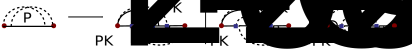
\includegraphics{KnottyPF/recursionP}
\end{equation}


For decomposing fragments like $PK_{l*O}$, in general $PK_{regex}$ it is now crucial to satisfy the band-decomposition-order constraint.
Let us start with the decomposition of $PK_{l*O}$. Generally $PK$-fragements are decomposed into $P_X$-type fragments, where we
need to allow recursive substructure (i.e. $WP$-fragments) between the $P_X$-fragments.

\begin{definition}
The structures represented by a $P_X$-type fragment over $[i..j]\cup [k..l]$ satisfy the following properties:
\begin{itemize}
\item all ends $i$, $j$, $k$, and $l$ are paired to something.
\item ``closed at $X$''---there is a base pair at the position $X$ ($X\in\{L,R,M,O\}$).
\item there is a base pair that spans the gap i region $j+1..k-1$
\item unless $X=O$, the ends cannot all be part of the same band. (Note that we terminate with O, unlike the original CCJ recursions, which terminate at M.)
\end{itemize}
\end{definition}


We obtain decompositions of PK-fragments like 
\begin{equation}
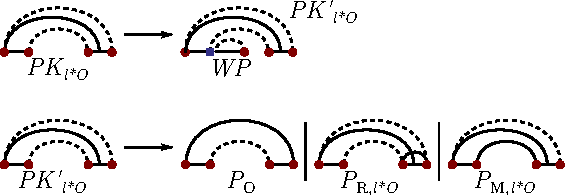
\includegraphics{KnottyPF/recursionPKlstarO}
\end{equation}
Note that the recursion to $P_O$ already satisfies the constraint due to $l*O$.

We need to further decompose the $P_X$ fragments (which are optionally restricted by regular expressions). Generally, we distinguish three cases by the type of the closing base pair at position $X$. 1) it could close an interior loop in the same band, 2) a multi-loop in the same band (with costs for inner base pairs and unpaired based accounted in WB), or 3) it could `close' the band, i.e. it is the innermost base pair of its band for bands at L,R,O---outermost, in the case of M. Note that the decomposition is disjoint. In the
third case, one changes to decomposing some other band (or terminates the final O-band). Also, in the third case, we allow recursive substructure between bands (WP), which needs to be inserted unambiguously.

Apart from some details in the unambiguous decomposition of multi-loops within bands (where the recursions operate on gapped fragments), it remains to ensure that the order in which bands are decomposed is never ambiguous. Note that in the handling of interior loops and multi-loops within a band, we can simply pass through any constraints on the order of band-decompositions.

\paragraph{Unambiguous decomposition order:}
The original CCJ algorithm already contains restrictions on the band-decomposition order, which are encoded in the rules for decomposition of $P\text{fromX}$-fragments ($X$ in $\{\text{L,R,M,O}\}$). These restrictions are
\begin{itemize}
\item (decomposition at) $R$ cannot be immediately followed by $L$
\item $M$ cannot be immediately followed by $O$
\item $O$ cannot be immediately followed by $M$
\end{itemize} 
The latter two restrictions ensure that the position changes correspond to true changes of the band (in both cases one would just extend the same band). The first restriction is indeed a disambiguation, since immediately successive decompositions at $L$ and $R$ could be exchanged, but it is again required to ensure that position changes introduce band changes, since going back and forth between $L$ and $R$ like $LRL$ would just extend the $L$ band. 

These restrictions in the original CCJ algorithm were necessary for proper scoring, but at the same time ensure unambiguous decomposition. 
%To see this, we go back to the properties of $P_X$-fragments:
%in each structure of a $P_X$-fragment (with the exception of the terminal O-band).


Here are examples for the decomposition of $P_X$:
\begin{equation}
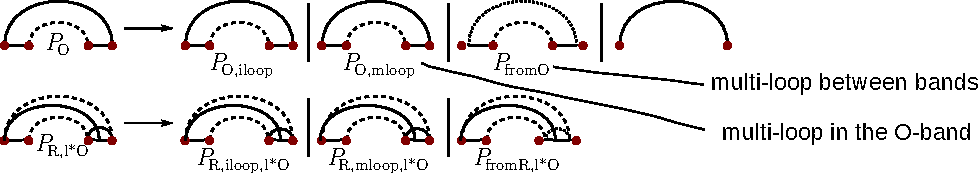
\includegraphics{KnottyPF/recursionPX}
\end{equation}

$P_{fromX}$-fragments are required to change the band; note that we need to unambiguously allow recursive substructure \emph{and} unambiguous band change. For the unconstrained $P_O$, the recursion to the unconstrained $P_\text{fromO}$ works like in the original recursions. 
\begin{equation}
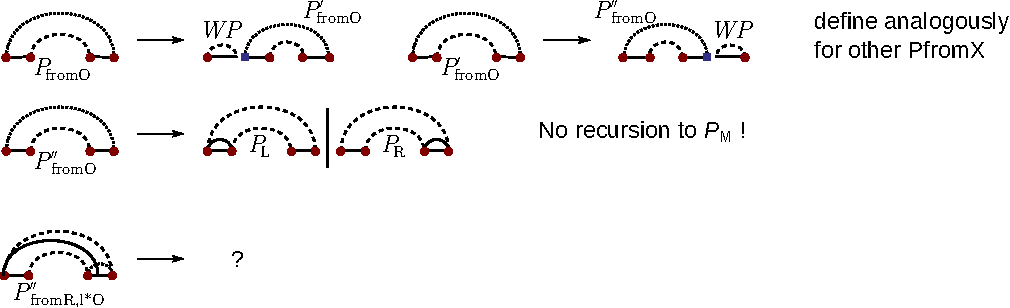
\includegraphics{KnottyPF/recursionPfromX}
\end{equation}
For the constrained case, we still need to work out all the details. Where to split off the WP-fragments? How to handle the $PK_{o*L}$-fragments (seems quite symmetric)?

\end{document}